\section{Contexts and Features}
\label{sec:framework}
%\hbadness=99999

Assuming that $\mathcal{Q}$ is the query log, a query $q \in \mathcal{Q}$ is a sequence of characters $q = (c_1^q, c_2^q, \ldots, c_i^q, \ldots, c_n^q)$. The external documents is a plain document set $\mathcal{D}$. For each character $c_i^q$ in $q$, we search in documents $\mathcal{D}$ and find its contexts. All the contexts of $c_i^q$ form a context bag $B_i$ which is a set of sentences. Given the context bag $B_i$, we design a simple but novel method to extract same kinds of features from each context and obtain the feature bag $F_i$.


\subsection{Context Searching}

For character $c_i^q$ in $q$, there are $4$ possible cases about its boundary information. $(1)$ $c_i^q$ is the begin and end of current segment, which means $c_i^q$ form a independent segment. The length of this segment is $1$. $(2)$ $c_i^q$ is the begin of current segment but not the end. The length of current segment is more than $1$. What's more, we can infer that the right bi-gram $c_i^qc_{i+1}^q$ of $c_i^q$ should belong to current segment. $(3)$ $c_i^q$ is the end of of current segment but not the begin. Also this segment is longer than $1$. And we know that the left bi-gram $c_{i-1}^q c_i^q$ should be in this segment. $(4)$ $c_i^q$ is in the middle position of current segment. This means tri-gram $c_{i_1}^q c_i^q c_{c+1}^q$ should be in this segment. In other words, left bi-gram is in one segment, and the same for right bi-gram. For case $(1)$ and $(2)$, the label of $c_i^q$ is ``B''. And for case $(3)$ and $(4)$, the label is ``I''.

%Statistic on segment length shows that more than $90\%$ segments is longer than $1$, which means case $(1)$ is relatively rare. Our context searching method is designed for $(2)$, $(3)$ and $(4)$.

From the view of left and right bi-grams, the existance of left bi-gram $c_{i_1}^q c_i^q$ indicates whethter $c_i^q$ is the begin of current segment, while the existance of right bi-gram indicates whether $c_i^q$ is the end of current segment. Because we do not know which bi-gram really exists, we search both two bi-grams in external documents $\mathcal{D}$. Sentences that contain any one of these two bi-gram are put into the context bag $B_i$. If a bi-gram exists, this bi-gram should be used frequently in documents. Therefore we can find many contexts which can support this bi-gram. Conversely, if a bi-gram does not exist, there should be few contexts which support this bi-gram. For example, in query ``高腰 / 连衣裙 / 白色'', the two bi-gram of character ``腰'' are ``高腰'' and ``腰连''. Because ``高腰'' is a common word in dress category, there are many contexts containing segment ``高腰'' in documents $\mathcal{D}$. ``腰连'' is not a common word in Chinese. Few contexts can be found to support ``腰连''. Further, we can make a conclusion that ``腰'' is case $(2)$. Note that there is no need to judge whether a context is found by left or right bi-gram. The distribution of contexts in context bag will decide the existance of these two bi-grams.


% For character $c_i^q$ in $q$, there are 3 possible cases about which segments it should belong to. $(1)$ $c_i^q$ is not the begin of a segment. Then $c_{i_1}^q c_i^q$ which is the left bi-gram of $c_i^q$ should be in same segment. $(2)$ $c_i^q$ is the begin of a segment, and the length of this segment is $1$. This means single $c_i^q$ form a independent segment. $(3)$ $c_i^q$ is the begin of a segment, and the length of this segment is longer than $1$. Therefore, $c_i^qc_{i+1}^q$ whic is the right bi-gram of $c_i^q$ should belong to same segment. Statistic on segment length shows that more than $90\%$ segments is longer than $1$, which means case $(2)$ is relatively rare. Our context search method is designed for case $(1)$ and $(3)$.


\subsection{Feature Extraction}

As we have mentioned, two nearest bi-grams are related to the boundary information of $c_i^q$. And we use these two bi-grams to search the contexts. We can also use the existance of these bi-grams in each contexts as boundary information. For example, a pair of boolean number $(1, 0)$ can be extract from a context. Number $1$ in the pair means the left bi-gram is mentioned in this context, while the $0$ in the pair indicates the right bi-gram is not mentioned. However, we design a novel method to extract the boundaries of $c_i^q$ in $q$, which is much more informative than the boolean pair.

The context bag $B_i$ is a set of sentences $(s_1, s_2, \ldots, s_j, \ldots)$. Each context must contain at least one of two bi-grams, $c_{i-1}^q c_i^q$ and $c_i^q c_{i+1}^q$. Therefore, $c_i^q$ must appear in any of these contexts. For each context, we treat $c_i^q$ as the center character, and apply same method to extract features. We use context $s_j$ in $B_i$ as example to illustrate how to extract the features. $s_j$ is a sequence of characters $(\ldots, c_{-3}^j, c_{-2}^j, c_{-1}^j, c_{0}^j, c_{+1}^j, c_{+2}^j, c_{+3}^j, \ldots)$ where $c_0^j$ is the center character and equal to $c_i^q$. Characters in the left of $c_0^j$ is called the left part, while characters in the right of $c_0^j$ is right part. We first align $s_j$ with the query $q$ according to $c_0^j$ in $s_j$ and $c_i^q$ in $q$. Then we subtract $q$ from $s_j$ character by character, which means we go through $s_j$ from center to two sides and take away the shared characters with $q$. Assuming the difference between $s_j$ and $q$ is $(\ldots, c_{-k_l-1}^j, c_{-k_l}^j, c_{0}^j, c_{+k_r}^j, c_{+k_r+1}^j, \ldots)$, where both characters between $c_{-k_l}^j$ and $c_{0}^j$ in left part and characters between $c_{+k_r}$ and $c_{0}^j$ in right part are token away. Figure \ref{fig:subtract} shows this process. The first line is a context of character ``衣''. The second line is the query. We algin the context and query by ``衣''. Character ``连'' and ``裙'' are token away. And both $k_l$ and $k_r$ are $2$.

\begin{figure}[th]
	\centering
	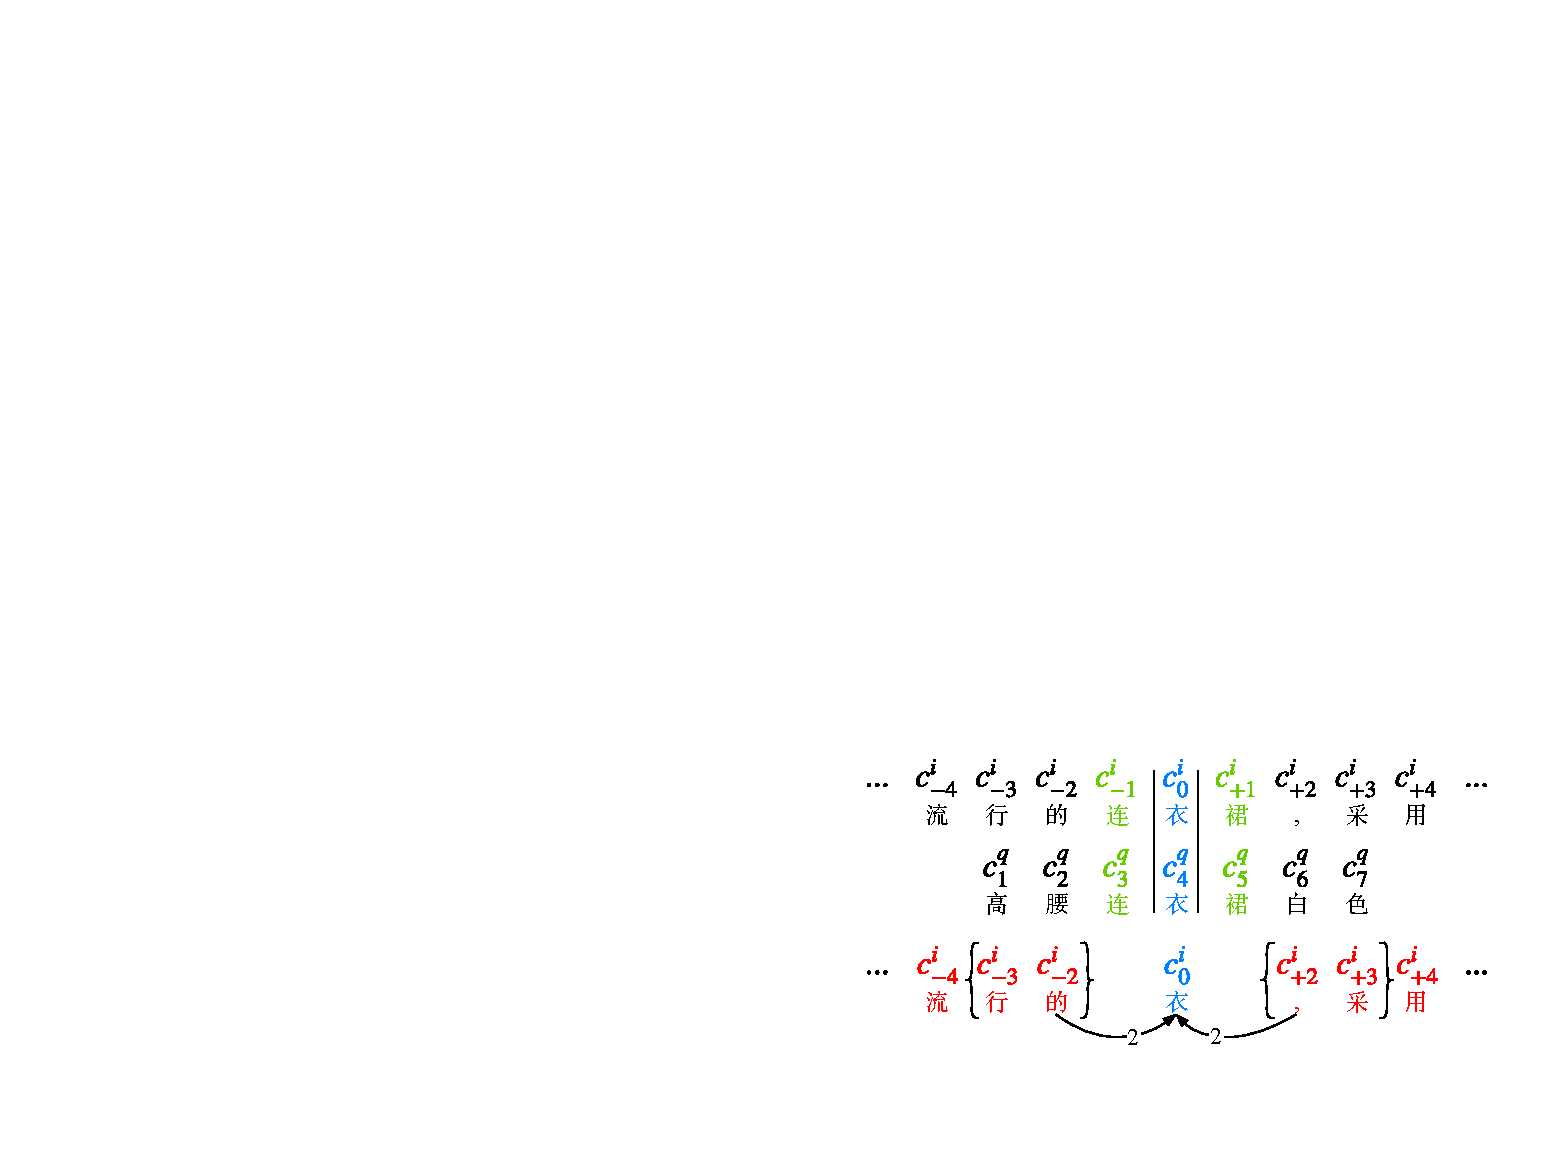
\includegraphics[width=0.9\columnwidth]{figures/lr.pdf}
	\caption{\small This is an example to show the process of extracting features. First line is one of the contexts of character ``衣''. Second line is the query. Third line is the subtraction result.}
	\label{fig:subtract}
	\vspace{-10pt}
\end{figure}

The left part of difference is used to extract features about left boundary of current segment, while the right part is for right boundary. Using left as example, $k_l$ can be treat as the distance between left boundary and the center character. In Figure \ref{fig:subtract}, $k_l$ is 2, which means there are $2$ characters (include center character itself) between the left boundary and center character ``衣''. Additionally, characters near the left boundary can also help to support current segment. When the window size is $2$, the left character features are $\{c_{-k_l-1}^j, c_{-k_l}^j \}$. In Figure \ref{fig:subtract}, left character features are $\{$``行", ``的" $\}$ where ``的'' is a typical stop signal in Chinese. As a conclusion, for left boundary, there are two kind of features, distance and character features. As for context $s_j$ of $c_i^q$, left feature $L_j$ is $(\{ c_{-k_l-1}^j, c_{-k_l}^j \}, k_l)$. Similarly, we can get right feature $R_j=(\{ c_{+k_r}^j, c_{+k_r+1}^j \}, k_r)$ which is for right boundary.

By appling above process to every context in context bag $B_i$, we can get the feature bag $F_i = (\left \langle L_1, R_1 \right \rangle, \left \langle L_2, R_2 \right \rangle, \cdots, \left \langle L_j, R_j \right \rangle, \cdots)$ where $\left \langle L_j, R_j \right \rangle$ is the features from context $s_j$. $F_i$ will be used to help to predict the label of $c_i^q$.

